\message{ !name(austin_report.tex)}\documentclass[11pt, letterpage]{article}
\usepackage{amsmath}
\usepackage{graphicx}

\begin{document}

\message{ !name(austin_report.tex) !offset(-3) }


\section{Selected Topics}
\subsection{Power Spectrum and Filtering}
To investigate the properties of the power spectrum and the effects of
filtering, we consider the simple discretely sampled sinusoidal signal:
\begin{equation}
  V_j = A \sin(2 \pi f t_j - \phi)
  \label{eq:sine}
\end{equation}

%%%%%%%%%%%%%%%%%%%%%%%%%%%%%%%%%%%%% 
% SHOW POWER IS CONFINED TO ONE BIN
%%%%%%%%%%%%%%%%%%%%%%%%%%%%%%%%%%%%%

\subsubsection{Power Spectra}
The power spectrum of a continuous signal is simply the square of the continuous
Fourier transform. However, when computing the power spectrum of a discretely
sampled signal, the leakage of power from some frequencies to others is a
problematic result of the digitization of the signal. To illustrate this, the
power spectra for two slightly different frequencies are considered: $f = 60$Hz
and $f = 59.673$Hz.

\begin{figure}
  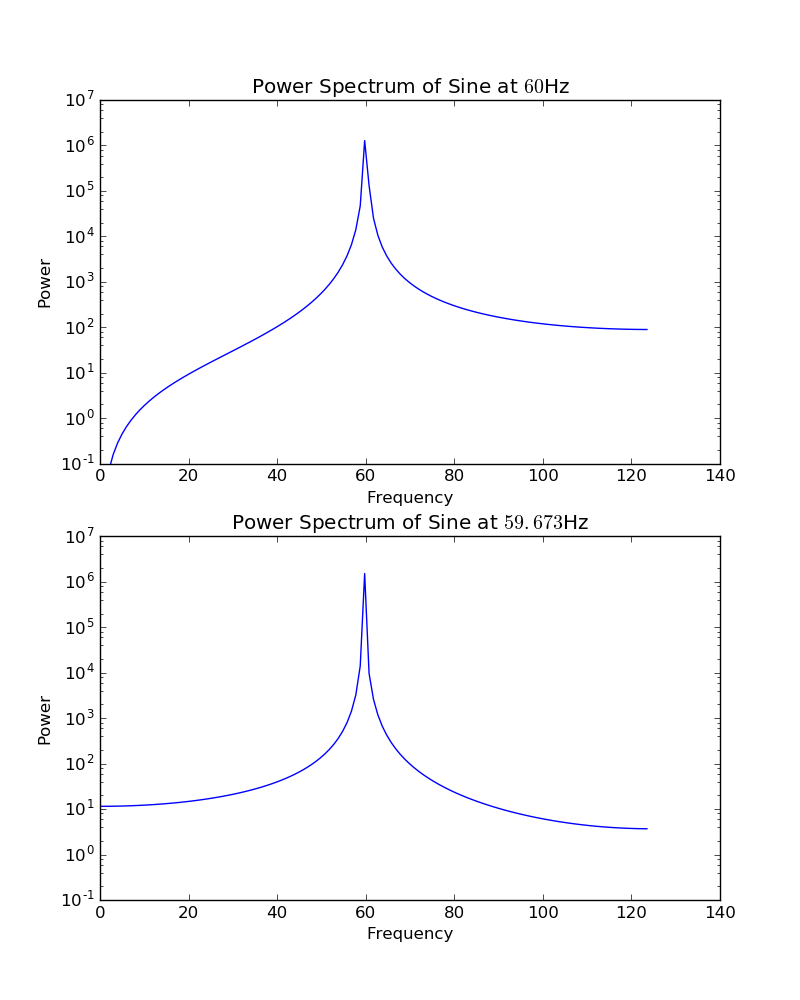
\includegraphics[width=\linewidth]{power_spectrum.png}
  \caption{
    The power spectra of equation \ref{eq:sine} with two very close frequencies.
  }
  \label{}
\end{figure}

\subsubsection{Windows}
One of the standard ways to reduce spectral leakage is to multiply the data in
time space with a window before performing the Fourier transform. Two of the
most common windows we look into are the Hann window and the Blackman-Harris
window. The Hann function and its Fourier transform are shown in figure
\ref{fig:hann_window}.

\begin{figure}
  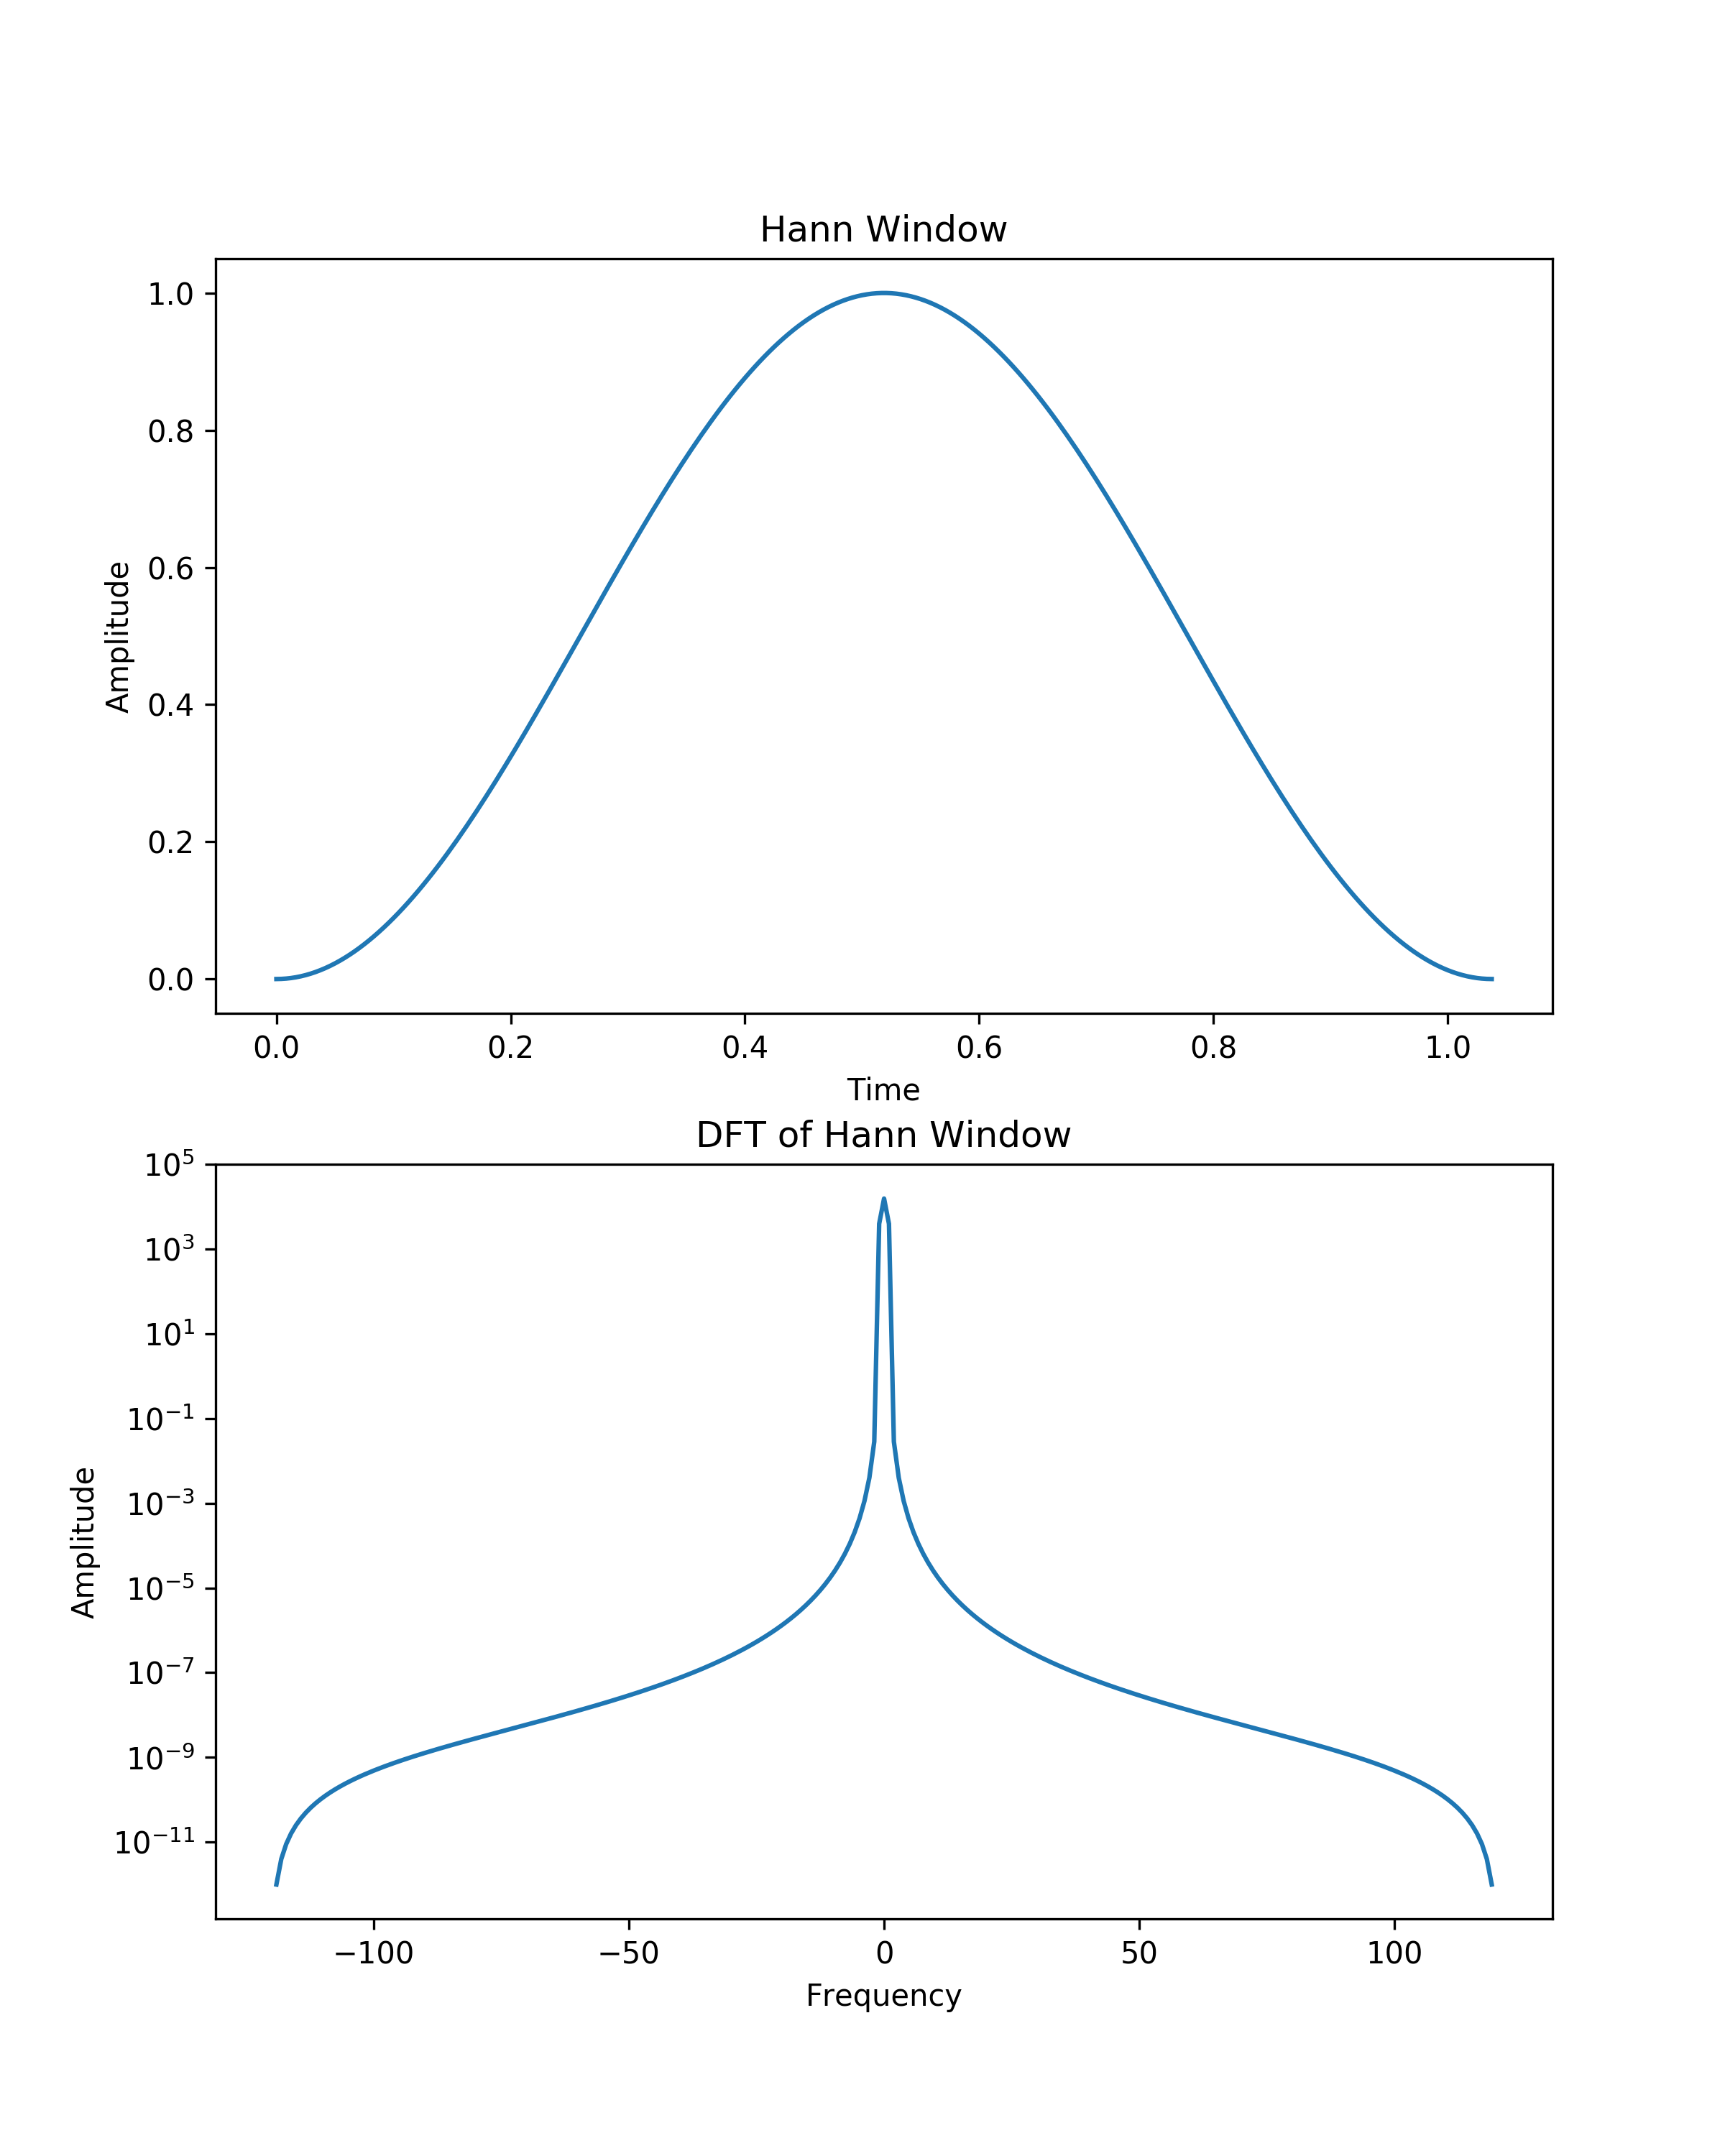
\includegraphics[width=\linewidth]{hann_window.png}
  \caption{
    The Hann window (top) and its Fourier transform (bottom). It can be thought
    of as a portion of a cosine wave.
  }
  \label{fig:hann_window}
\end{figure}

Now the Hann window can be applied to the two signals that were used previously
with frequencies $60$Hz and $59.673$Hz, shown in figures \ref{fig:hann_0} and
\ref{fig:hann_1}, respectively. 

\begin{figure}
  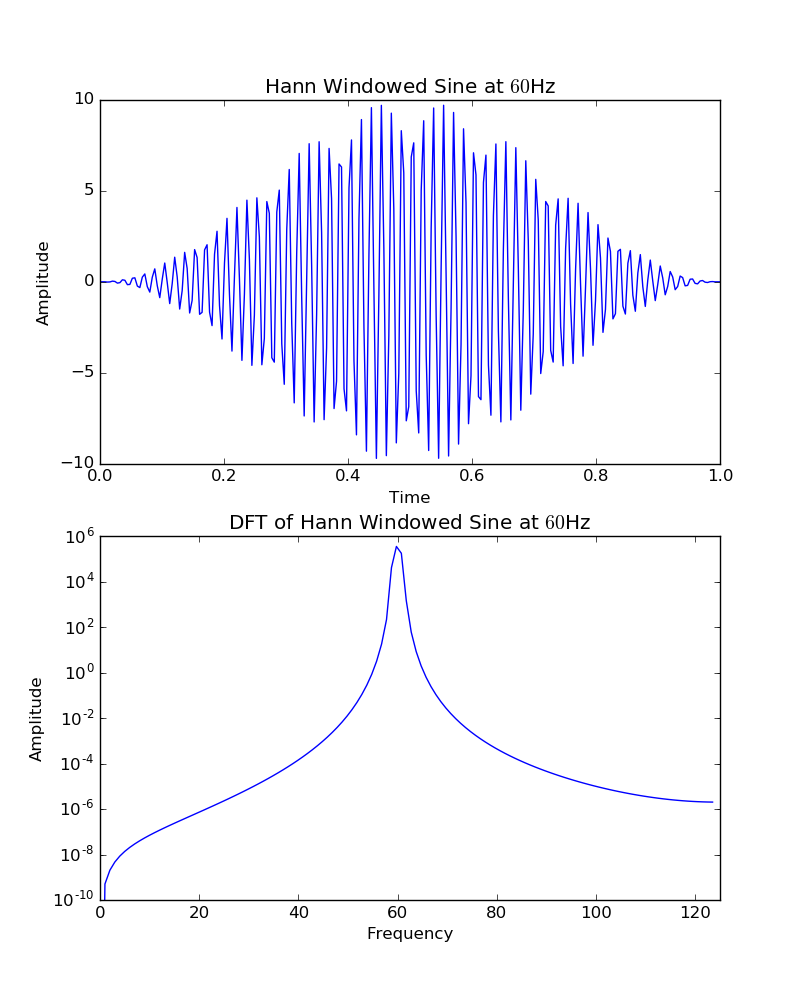
\includegraphics[width=\linewidth]{hann_0.png}
  \caption{
    The Hann window applied to equation \ref{eq:sine} with $f = 60$Hz in time
    space (top) and in frequency space (bottom).
  }
  \label{fig:hann_0}
\end{figure}

\begin{figure}
  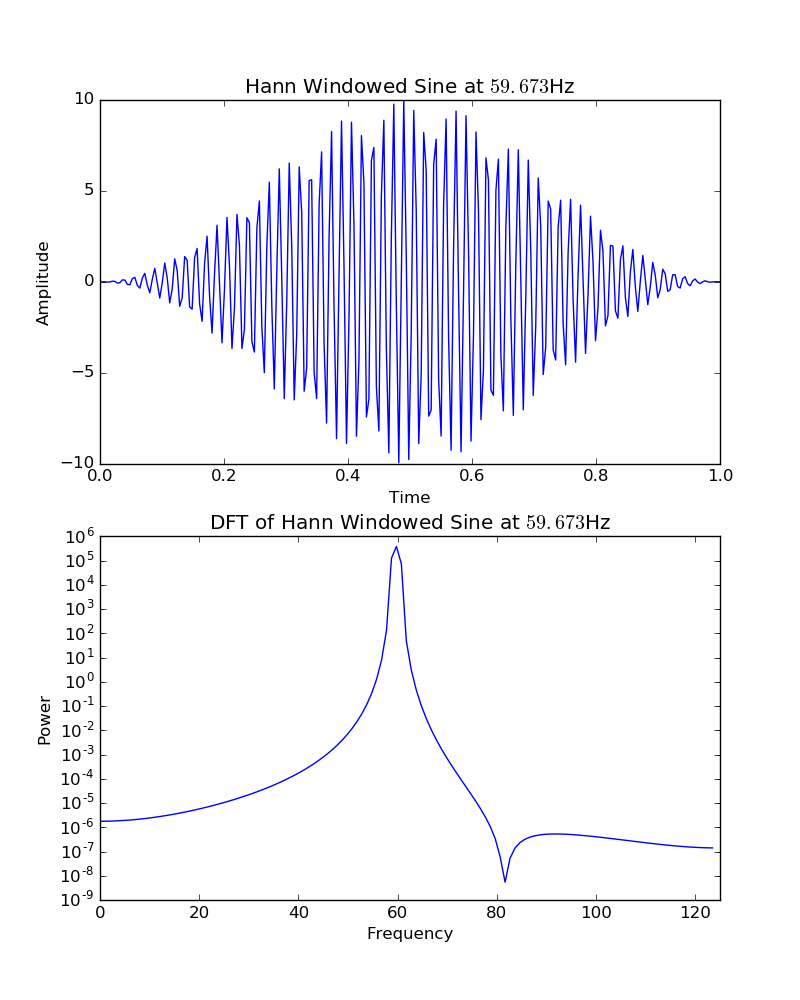
\includegraphics[width=\linewidth]{hann_1.png}
  \caption{
    The Hann window applied to equation \ref{eq:sine} with $f = 59.673$Hz in
    time space (top) and in frequency space (bottom).
  }
  \label{fig:hann_1}
\end{figure}


\end{document}
\message{ !name(austin_report.tex) !offset(-79) }
